\section{Synthesis my design}

Tiến hành sử dụng file .tcl sau để thực hiện trên Genus:

\begin{lstlisting}[style=StyleCode, language=TCL, caption={genus\_synthesis.tcl}]
	
	##################################################
	#
	# EE3213_04 (cre: Khai Pham)
	# Digital system design and Verification
	#
	##################################################
	set Top_module  FPU_unit
	set LIB_DIR     "./../PDK45nm/gpdk045_lib"
	set LIB_NAME    "fast_vdd1v0_basicCells_hvt"
	set LIB_FILE    "${LIB_DIR}/${LIB_NAME}.lib"
	set SDC_FILE    "./constraint.sdc"
	set SRC_FILE    "./../../02_rtl/"
	if {![file exists ${LIB_FILE}]} {
		error "ERROR: Library file not found: ${LIB_FILE}"
	}
	put "TOP_MODULE = $Top_module"
	put "LIB_DIR = $LIB_DIR"
	put "LIB_NAME = $LIB_NAME"
	put "LIB_FILE = $LIB_FILE"
	put "SDC_FILE = $SDC_FILE"
	put "SRD_FILE = $SRC_FILE"

	read_libs ${LIB_FILE}
	read_hdl -sv [glob ${SRC_FILE}*.sv]
	elaborate
	set_top_module ${Top_module}

	set elab_v "./${LIB_NAME}/${Top_module}_elab.v"
	write_hdl > ${elab_v}
	check_design -all

	read_sdc ${SDC_FILE}

	set_db syn_generic_effort medium
	set_db syn_map_effort medium 
	set_db syn_opt_effort medium

	syn_generic
	set generic_v "./${LIB_NAME}/${Top_module}_generic.v"
	write_hdl > ${generic_v}

	syn_map
	set techmap_v "./${LIB_NAME}/${Top_module}_tech_map.v"
	write_hdl > $techmap_v

	remove_assigns_without_optimization -verbose
	syn_opt

	report timing -lint
	set netlist_v "./${LIB_NAME}/${Top_module}_netlist.v"
	write_hdl > ${netlist_v}

	set sdf_out "./${LIB_NAME}/${Top_module}.sdf"
	write_sdf -timescale ns -nonegchecks -recrem split -edges check_edge -setuphold split  > $sdf_out

	report_timing -max_paths 1 > ./${LIB_NAME}/report/${Top_module}_timing.rpt
	report hierarchy > ./${LIB_NAME}/report/${Top_module}_hier.rpt
	report gates > ./${LIB_NAME}/report/${Top_module}_gates.rpt
	report datapath > ./${LIB_NAME}/report/${Top_module}_datapath.rpt
	report_qor > ./${LIB_NAME}/report/${Top_module}_qor.rpt
	report_area > ./${LIB_NAME}/report/${Top_module}_area.rpt
	report_power > ./${LIB_NAME}/report/${Top_module}_power.rpt

	puts "Done. Using library: $LIB_FILE"
	puts "Elaborated    -> $elab_v"
	puts "Generic       -> $generic_v"
	puts "Tech-mapped   -> $techmap_v"
	puts "Netlist       -> $netlist_v"
	puts "SDF           -> $sdf_out"
	puts "Reports       -> ./${LIB_NAME}/report/"

	##################################################
	# Open genus GUI
	gui_show
\end{lstlisting}

Với file \textbf{constraint.sdc} như sau:

\begin{lstlisting}[style=StyleCode, language=TCL, caption={File constraint.sdc}]
	set_max_delay ?.0 -from [all_inputs] -to [all_outputs]
	set_input_delay 0.1 -clock [get_clocks *] [all_inputs]
	set_output_delay 0.1 -clock [get_clocks *] [all_outputs]
	set timing_report_unconstrained true
\end{lstlisting}

\begin{enumerate}[label=\arabic*.]
	\item Kết quả của \textbf{timing.rpt} như sau:
		\begin{itemize}
			\item \textbf{slow\_vdd1v2\_basicCells\_lvt.lib}:
				% TODO: \usepackage{graphicx} required
				\begin{figure}[H]
					\centering
					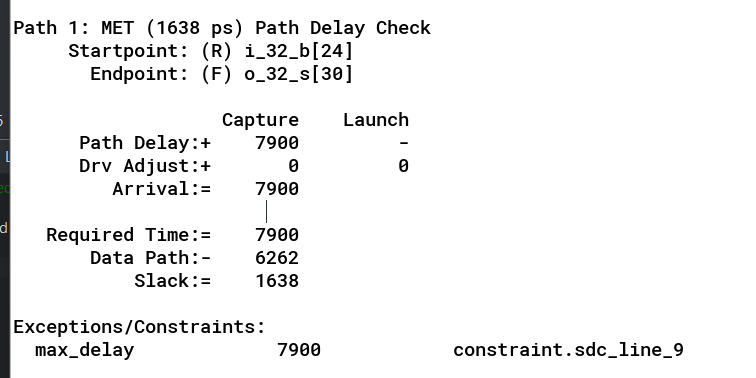
\includegraphics[width=0.7\linewidth]{my-chapters/my-images/timing/screenshot001}
					\caption{}
					\label{fig:screenshot001}
				\end{figure}
				
			
			\item \textbf{slow\_vdd1v2\_basicCells\_hvt.lib}:
				% TODO: \usepackage{graphicx} required
				\begin{figure}[H]
					\centering
					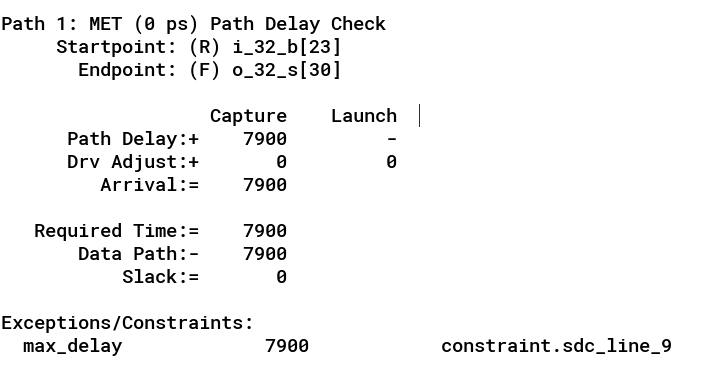
\includegraphics[width=0.7\linewidth]{my-chapters/my-images/timing/screenshot002}
					\caption{}
					\label{fig:screenshot002}
				\end{figure}
				
		
			\item \textbf{slow\_vdd1v0\_basicCells\_lvt.lib}:
				% TODO: \usepackage{graphicx} required
				\begin{figure}[H]
					\centering
					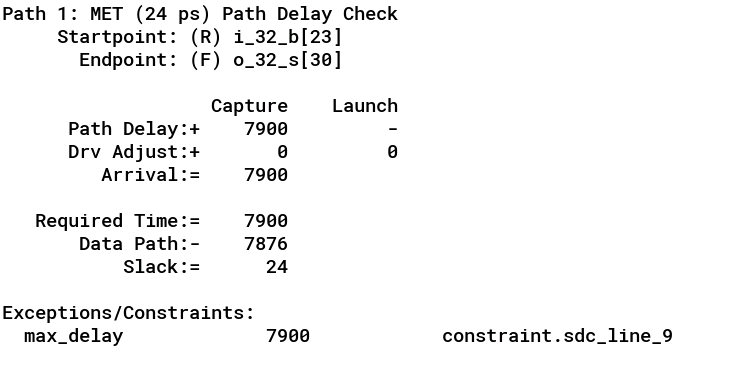
\includegraphics[width=0.7\linewidth]{my-chapters/my-images/timing/screenshot003}
					\caption{}
					\label{fig:screenshot003}
				\end{figure}
				
			
			\item \textbf{slow\_vdd1v0\_basicCells\_hvt.lib}:
				% TODO: \usepackage{graphicx} required
				\begin{figure}[H]
					\centering
					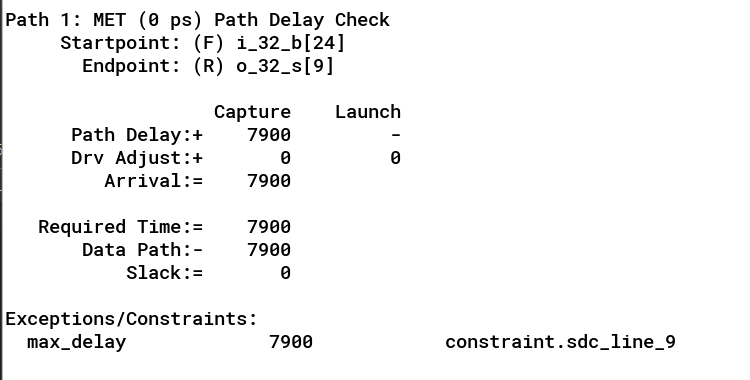
\includegraphics[width=0.7\linewidth]{my-chapters/my-images/timing/screenshot004}
					\caption{}
					\label{fig:screenshot004}
				\end{figure}
				
			
			\item \textbf{fast\_vdd1v2\_basicCells\_lvt.lib}:
				% TODO: \usepackage{graphicx} required
				\begin{figure}[H]
					\centering
					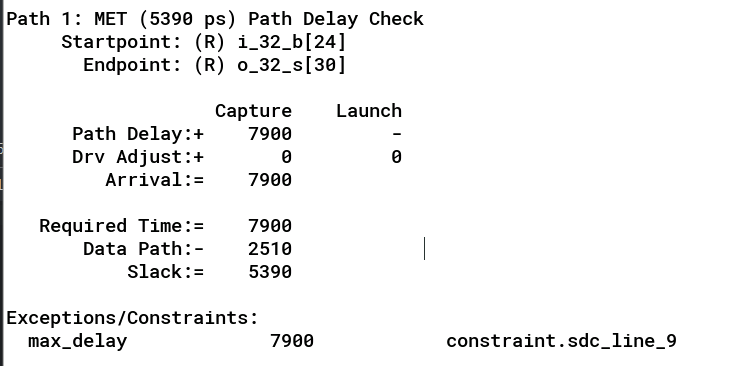
\includegraphics[width=0.7\linewidth]{my-chapters/my-images/timing/screenshot005}
					\caption{}
					\label{fig:screenshot005}
				\end{figure}
				
			
			\item \textbf{fast\_vdd1v2\_basicCells\_hvt.lib}:
				% TODO: \usepackage{graphicx} required
				\begin{figure}[H]
					\centering
					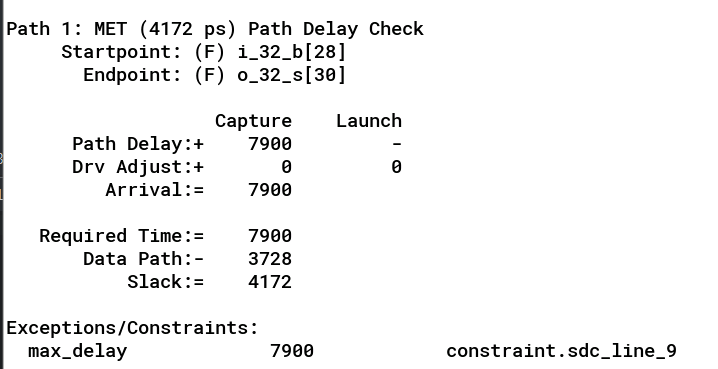
\includegraphics[width=0.7\linewidth]{my-chapters/my-images/timing/screenshot006}
					\caption{}
					\label{fig:screenshot006}
				\end{figure}
				
			
			\item \textbf{fast\_vdd1v0\_basicCells\_lvt.lib}:
				% TODO: \usepackage{graphicx} required
				\begin{figure}[H]
					\centering
					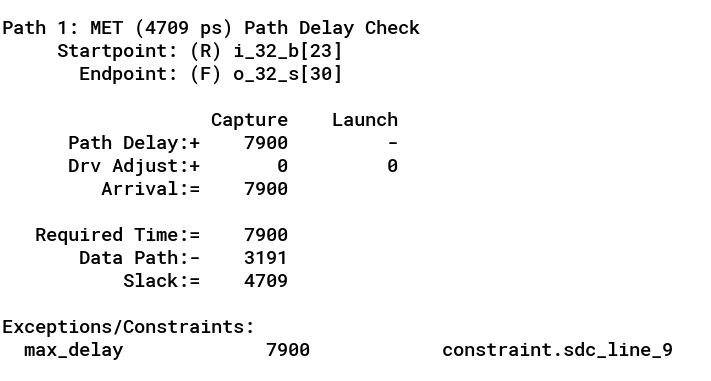
\includegraphics[width=0.7\linewidth]{my-chapters/my-images/timing/screenshot007}
					\caption{}
					\label{fig:screenshot007}
				\end{figure}
				
			
			\item \textbf{fast\_vdd1v0\_basicCells\_hvt.lib}:
				% TODO: \usepackage{graphicx} required
				\begin{figure}[H]
					\centering
					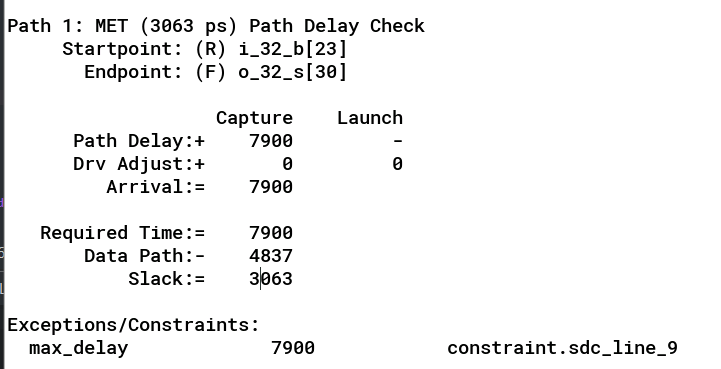
\includegraphics[width=0.7\linewidth]{my-chapters/my-images/timing/screenshot008}
					\caption{}
					\label{fig:screenshot008}
				\end{figure}
				
		\end{itemize}
	\item Kết quả của Synthesis:
		\begin{figure}[H]
			\centering
			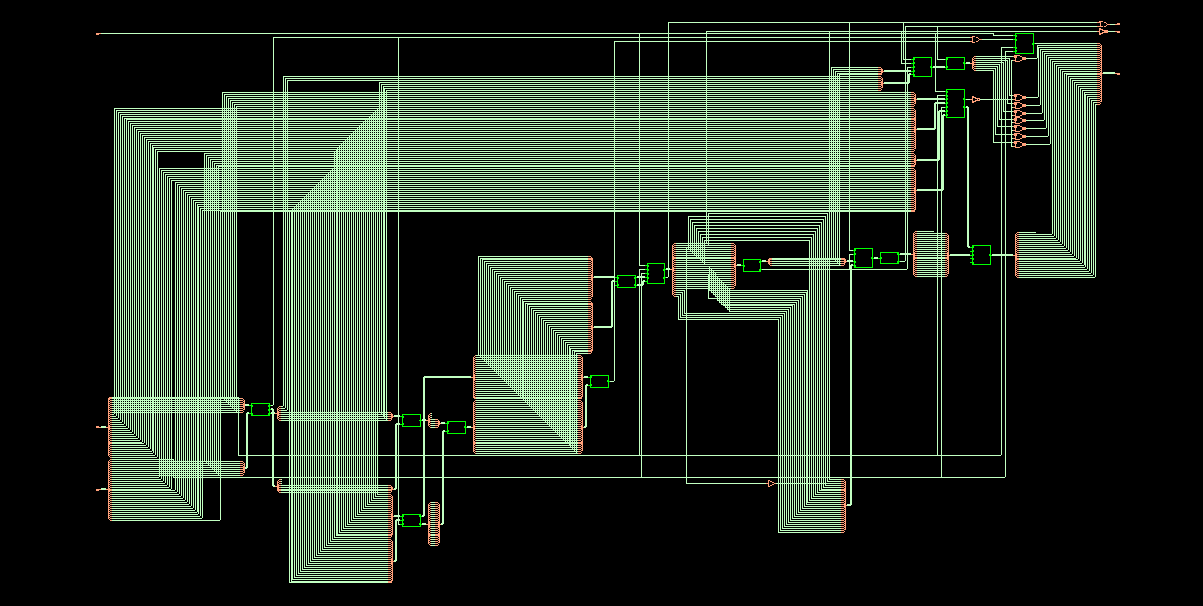
\includegraphics[width=\linewidth]{./my-chapters/my-images/synthesis/block_diagram_synthesis.png}
		\end{figure}
\end{enumerate}
